%%%%%%%%%%%%%%%%%%%%%%%%%%%%%%%%%%%%%%%%%%%%%%%%%%%%%%%%%%%%%%%%%%%%%%%%%%%%%%%
%% El Entorno de R
%%%%%%%%%%%%%%%%%%%%%%%%%%%%%%%%%%%%%%%%%%%%%%%%%%%%%%%%%%%%%%%%%%%%%%%%%%%%%%%
\chapter{El entorno de R}

Este capítulo comprende algunos aspectos prácticos del trabajo con \textbf{R}.
Describe cuestiones relacionadas con la estructura del espacio de trabajo, los
dispositivos gráficos y sus parámetros, y la programación elemental, e incluye
una discusión bastante extensa, aunque lejos de ser completa, sobre el ingreso
de datos.

%%%%%%%%%%%%%%%%%%%%%%%%%%%%%%%%%%%%%%%%%%%%%%%%%%%%%%%%%%%%%%%%%%%%%%%%%%%%%%%
\section{Administración de sesiones}
%%%%%%%%%%%%%%%%%%%%%%%%%%%%%%%%%%%%%%%%%%%%%%%%%%%%%%%%%%%%%%%%%%%%%%%%%%%%%%%

%%%%%%%%%%%%%%%%%%%%%%%%%%%%%%%%%%%%%%%%%%%%%%%%%%%%%%%%%%%%%%%%%%%%%%%%%%%%%%%
\subsection{El espacio de trabajo}
%%%%%%%%%%%%%%%%%%%%%%%%%%%%%%%%%%%%%%%%%%%%%%%%%%%%%%%%%%%%%%%%%%%%%%%%%%%%%%%

Todas las variables creadas en R se almacenan en un espacio de trabajo común.
Para ver qué variables están definidas en el área de trabajo, puede utilizar la
función \texttt{ls} (lista).  Si ha ejecutado todos los ejemplos del capítulo
anterior es posible que la salida sea similar a esto:

\begin{lstlisting}[language=R]
> ls()
 [1] "bmi"           "d"             "exp.lean"      "exp.obese"    
 [5] "fpain"         "height"        "hh"            "intake.post"  
 [9] "intake.pre"    "intake.sorted" "l"             "m"            
[13] "mylist"        "o"             "oops"          "pain"         
[17] "sel"           "v"             "weight"        "x"            
[21] "xbar"          "y"   
\end{lstlisting}

Recuerde no omitir los paréntesis al invocar a \texttt{ls}().

Si en algún momento las cosas comienzan a ser confusas, podemos eliminar
algunos objetos del entorno. Esto se puede hacer mediante \texttt{rm}()
(remover), de manera que:

\begin{lstlisting}[language=R]
> rm(height, weight)
\end{lstlisting}

Elimina las variables \texttt{height} y \texttt{weight}.

Se puede eliminar completamente el espacio de trabajo mediante
\texttt{rm(list=ls())}, y también mediante la opciones de menú “Remove all
objects” o “Clear Workspace” en las versiones graficas de \textbf{R}. Esto no
elimina las variables cuyo nombre comienza con un punto (\texttt{.}) por que
las mismas no son listadas por \texttt{ls()} - necesitaríamos usa
\texttt{ls(all=T)} para eso,  pero podría ser peligros ya que algunos objetos
usados por el sistema usan esta notación.

Si está familiarizado con el sistema operativo \textbf{Unix}, para el cual el
lenguaje \textbf{S}, que precedió a \textbf{R}, fue escrito originalmente,
entonces sabrá que los comandos para listar y eliminar archivos en Unix se
llaman precisamente \texttt{ls} y \texttt{rm}.

Es posible salvar completamente el espacio de trabajo en cualquier momento.
Simplemente deberemos escribir:

\begin{lstlisting}[language=R]
> save.image()
\end{lstlisting}

de esta forma, todo será salvado en un archivo de nombre \texttt{.RData} en el
directorio de trabajo actual. Las versiones gráficas también tienen un menú
para hacer esto. Cuando salimos de \textbf{R} se nos puede llegar a preguntar
si queremos salvar una imagen de nuestro espacio de trabajo; si le decimos que
sí estaremos haciendo exactamente lo mismo. Es posible también especificar un
nombre de archivo a salvar alternativo (usando comillas), también podremos
salvar objetos específicos con \texttt{save}. El archivo \texttt{.RData} se
carga automáticamente cuando se inicia \texttt{R} desde el directorio dónde se
encuentre. Otros archivos similares pueden cargarse al espacio de trabajo
mediante \texttt{load}.

%%%%%%%%%%%%%%%%%%%%%%%%%%%%%%%%%%%%%%%%%%%%%%%%%%%%%%%%%%%%%%%%%%%%%%%%%%%%%%%
\subsection{Salida Textual}
%%%%%%%%%%%%%%%%%%%%%%%%%%%%%%%%%%%%%%%%%%%%%%%%%%%%%%%%%%%%%%%%%%%%%%%%%%%%%%%

Es importante tener en cuenta que el espacio de trabajo está formado únicamente
por objetos \textbf{R}, no por ninguna de las salidas generadas durante la
sesión de trabajo.  Si desea guardar ésta utilice "Guardar en archivo" en el
menú Archivo de la versión Gráfica o utilice las funciones estándar de cortar y
pegar. También puede utilizar \textbf{ESS} (Emacs Speaks Statistics), que
funciona en todas las plataformas. Es un "modo" para el editor \textbf{Emacs}
en el que puede ejecutar toda la sesión en un búfer. Puede obtener la
\textbf{ESS} y las instrucciones de instalación de \textbf{CRAN} (ver Apéndice
A).  

Una forma alternativa de redirigir la salida a un archivo es usar la función
\texttt{sink}. Se trata en gran medida de una reliquia de la época de las
terminales de 80 x 25, en la que no se disponía de técnicas de cortar y pegar,
pero que aún puede ser útil en ocasiones. En particular, se puede utilizar en
el procesamiento por lotes. La forma en que funciona es de la siguiente manera:

\begin{lstlisting}[language=R]
> sink("salidatxt")
> ls()
\end{lstlisting}

No aparece ninguna salida por pantalla!. Esto por que ahora la salida normal de
cualquier comando o función se redirige automáticamente al archivo
\texttt{salida.txt} en el directorio actual.  El sistema permanecerá trabajando
de esta forma hasta que ejecutemos nuevamente (esta vez sin parámetros):

\begin{lstlisting}[language=R]
> sink()
\end{lstlisting}

El directorio de trabajo actual se puede obtener mediante \texttt{getwd()} y
establecer otro mediante \texttt{setwd(mi directorio)}, dónde \texttt{mi
directorio} es una cadena de texto. El directorio de trabajo inicial depende
del sistema, por ejemplo para las versiones gráficas suele ser el \texttt{home
dir} del usuario y en la versión de línea de comandos es la carpeta desde dónde
se ha ejecutado \textbf{R}.

%%%%%%%%%%%%%%%%%%%%%%%%%%%%%%%%%%%%%%%%%%%%%%%%%%%%%%%%%%%%%%%%%%%%%%%%%%%%%%%
\subsection{Scripting}
%%%%%%%%%%%%%%%%%%%%%%%%%%%%%%%%%%%%%%%%%%%%%%%%%%%%%%%%%%%%%%%%%%%%%%%%%%%%%%%

Más allá de un cierto nivel de complejidad, seguramente no querrá trabajar con
\textbf{R} línea por línea. En estas situaciones, es mejor trabajar con scripts
\textbf{R}, colecciones de líneas de código almacenadas en un archivo o en la
memoria de la computadora de alguna forma. 

Una opción es usar la función de \texttt{source}, que es algo así como lo
opuesto a \texttt{sink}. Toma la entrada (es decir, los comandos desde un
archivo) y los ejecuta. Nótese, sin embargo, que todo el archivo se comprueba
sintácticamente antes de que ejecutar cualquier instrucción. A menudo es útil
configurar \texttt{echo=T} en la llamada para que los comandos sean impresos
junto con la salida. 

Otra opción es de naturaleza más interactiva. Puedes trabajar con un editor que
le permite enviar una o más líneas del script a una instancia de R en
ejecución, el cual se comportará como si las mismas líneas hubieran sido
introducida en el indicador de comandos. Las versiones de Windows, Linux y
Macintosh de R tienen ventanas de scripting simples incorporadas, y un número
importante de Editores de texto tienen la funcionalidad para enviar los
comandos a R.

\begin{tradnote} 
	
	Actualmente son muchas las herramientas para trabajar en R, muchas más de
	las que existían al momento de la publicación original de este libro. En
	lineas generales hoy tenemos R en las tres principales plataformas:
	Windows, Linux y MAC, en cada una además podemos contar con:

	\begin{description}
	\item[$\bullet$] Interprete interactivo por línea de comando (\texttt{R})
	\item[$\bullet$] Versión grafica (\texttt{Rgui})
	\item[$\bullet$] Múltiples editores de texto con integración con \textbf{R}
	\item[$\bullet$] Entornos integrados de desarrollo (\textbf{Rstudio})
	\end{description}

\end{tradnote}

El historial de los comandos introducidos en una sesión se puede guardar y
volver a cargar utilizando los comandos \texttt{savehistory} y
\texttt{loadhistory}, que también se asignan a entradas de menú en la versión
gráfica. Las comandos guardados pueden ser útiles como punto de partida para
escribir scripts; observe también que la función \texttt{history()} mostrará
los últimos comandos introducidos en la consola (hasta un máximo de 25 líneas
por defecto)

%%%%%%%%%%%%%%%%%%%%%%%%%%%%%%%%%%%%%%%%%%%%%%%%%%%%%%%%%%%%%%%%%%%%%%%%%%%%%%%
\subsection{El sistema de ayuda de R}
%%%%%%%%%%%%%%%%%%%%%%%%%%%%%%%%%%%%%%%%%%%%%%%%%%%%%%%%%%%%%%%%%%%%%%%%%%%%%%%

\textbf{R} puede hacer mucho más de lo que un principiante podría llegar a
necesitar o incluso entender. Este libro está escrito de tal manera que la
mayor parte del código que probablemente necesitará en relación con los
procedimientos estadísticos se describe en el texto, y el compendio en el
Apéndice C está diseñado para proporcionar una visión general básica. Sin
embargo, es evidente que no es posible abarcar todo.  

\textbf{R} también viene con una amplia ayuda en línea en forma de texto, así
como en forma de una serie de archivos HTML que se pueden leer utilizando
cualquier navegador Web Se puede acceder a las páginas de ayuda a través de
``help'' en la barra de menú de Windows e introduciendo \texttt{help.start()} en
cualquier plataforma. Encontrará que las páginas son de naturaleza técnica. La
precisión y la concisión prevalecen aquí sobre la legibilidad y la pedagogía
(algo que se aprende a apreciar después de la exposición a lo contrario).  

Desde la línea de comandos, siempre puede introducir \texttt{help(aggregate)}
para obtener ayuda de la función \texttt{aggregate} o utilizar el prefijo
\texttt{?}, por ejemplo: \texttt{?aggregate}. Si el visor de HTML se está
ejecutando, entonces la página de ayuda se mostrará allí. De lo contrario, se
mostrará como texto en un misma ventana del terminal o en una ventana separada.
Tenga en cuenta que la versión HTML del sistema de ayuda incluye un ``Motor de
búsqueda y claves'' muy útil y que la función \texttt{apropos} le permite
obtener una lista de nombres de comandos que contienen un patrón dado. La
función \texttt{help.search} es similar, pero utiliza coincidencias difusas y
busca más profundamente en las páginas de ayuda, de modo que podrá localizar,
por ejemplo, el coeficiente de correlación de Kendall en \texttt{cor.test} si
utiliza \texttt{help.search("kendal")}. 

También está disponible con las distribuciones de \textbf{R}, un conjunto de
documentos en varios formatos. Es particularmente interesante ``An Introduction
to R'', basado originalmente en una serie de notas para \textbf{S-PLUS} de Bill
Venables y David Smith y adaptado a \textbf{R} por varias personas.  Contiene
una introducción al lenguaje \textbf{R} y al entorno, mucho más centrada en el
lenguaje en sí que este libro. En la plataforma Windows, puede elegir instalar
documentos PDF como parte del procedimiento normal de instalación para poder
acceder luego por medio del menú ``Ayuda''.  Se puede acceder también a una
versión HTML (sin imágenes) a través del navegador en todas las plataformas.

%%%%%%%%%%%%%%%%%%%%%%%%%%%%%%%%%%%%%%%%%%%%%%%%%%%%%%%%%%%%%%%%%%%%%%%%%%%%%%%
\subsection{Paquetes}\label{paquetes}
%%%%%%%%%%%%%%%%%%%%%%%%%%%%%%%%%%%%%%%%%%%%%%%%%%%%%%%%%%%%%%%%%%%%%%%%%%%%%%%

Una instalación de \texttt{R} contiene una o más librerías o paquetes. Algunos
de estos paquetes forman parte de la instalación básica.  Otros pueden ser
descargados desde \textbf{CRAN} (ver apéndice A), el cual alberga a la fecha
más de 12000 paquetes para múltiples propósitos.  Incluso podríamos crear
nuestros propios paquetes. Una librería es por lo general una simple carpeta en
el disco. Una librería de sistema se crea al instalar \texttt{R}.  En algunas
instalaciones, no les es permitido a los usuarios modificar la librería del
sistema. De todas formas, es posible configurara librerías privadas; para más
detalles ver \texttt{help(".Library")}.

Un paquete puede contener, funciones escritas en \textbf{R}, librerías de carga
dinámica escritas en \textbf{C} o \textbf{Fortran} y distintos conjuntos de
datos.  Un paquete generalmente implementa funcionalidad que la mayoría de los
usuarios probablemente no necesiten tener cargada todo el tiempo. Un paquete es
cargado en \textbf{R} mediante el comando \texttt{library}, de esta forma, para
cargar el paquete \texttt{survival} tendremos que ingresar:

\begin{lstlisting}[language=R]
> library(survival)
\end{lstlisting}

Los paquetes cargados, no se consideran parte del espacio de trabajo. Si
terminamos la sesión \texttt{R} y comenzamos una nueva con es espacio de
trabajo guardado, deberemos cargar nuevamente los paquetes anteriores.  Por
esta misma razón, rara vez necesitemos descargar un paquete activo, pero si lo
llegaremos a necesitar hacer, podríamos escribir:

\begin{lstlisting}[language=R]
> detach("package:survival")
\end{lstlisting}

(ver sección \ref{attachdetach}.)

%%%%%%%%%%%%%%%%%%%%%%%%%%%%%%%%%%%%%%%%%%%%%%%%%%%%%%%%%%%%%%%%%%%%%%%%%%%%%%%
\subsection{Datos integrados}
%%%%%%%%%%%%%%%%%%%%%%%%%%%%%%%%%%%%%%%%%%%%%%%%%%%%%%%%%%%%%%%%%%%%%%%%%%%%%%%

Muchos paquetes, tanto dentro como fuera de la distribución R estándar, vienen
con algún que otro conjunto de datos incorporado. Estos conjuntos de datos
pueden ser bastante grandes, por lo que no es una buena idea mantenerlos en la
memoria en todo momento. Se requiere entonces, un mecanismo para la carga bajo
demanda. En muchos paquetes, esto funciona a través de un mecanismo llamado
\textit{carga perezosa} ("lazy loading,"), que permite al sistema "simular" que
los datos están sí  en memoria, pero en realidad no se cargan hasta que son
referenciados por primera vez.  

Con este mecanismo, los datos están al alcance de la mano. Por ejemplo, si
escribe \texttt{thuesen}, se muestra el \texttt{data.frame} de dicho nombre.
Algunos paquetes todavía requieren llamadas explícitas a la función
\texttt{data}.  La mayoría de las veces, esto carga un \texttt{data.frame} con
el nombre que se especifica como parámetro; \texttt{data(thuesen)}, por
ejemplo, carga el \texttt{data.frame} "thuesen".

Lo que hace \texttt{data} es recorrer los directorios de datos asociados a cada
paquete (ver Sección \ref{paquetes}) y buscar archivos cuyo nombre base
coincida con el nombre especificado. Dependiendo de la extensión del archivo,
pueden suceder varias cosas. Los archivos con extensión \texttt{.tab} se leen
usando \texttt{read.table} (Sección \ref{readtextfile}), mientras que los
archivos con extensión \texttt{.R} se ejecutan como archivos de código (¡y
podrían, en general, hacer cualquier cosa!), esto simplemente, por dar dos
ejemplos comunes.

Si hay un subdirectorio del directorio actual llamado \texttt{data}, entonces
también se busca en él. Esta puede ser una forma muy útil de organizar sus
proyectos personales.

%%%%%%%%%%%%%%%%%%%%%%%%%%%%%%%%%%%%%%%%%%%%%%%%%%%%%%%%%%%%%%%%%%%%%%%%%%%%%%%
\subsection{\texttt{attach} y \texttt{detach}}\label{attachdetach}
%%%%%%%%%%%%%%%%%%%%%%%%%%%%%%%%%%%%%%%%%%%%%%%%%%%%%%%%%%%%%%%%%%%%%%%%%%%%%%%

La notación para acceder a variables en \texttt{data.frames} se vuelve bastante pesada
si tiene que escribir repetidamente comandos largos como:

\begin{lstlisting}[language=R]
> plot(thuesen$blood.glucose,thuesen$short.velocity)
\end{lstlisting}

Afortunadamente, puede hacer que\textbf{R} busque objetos entre las variables
de un \texttt{data.frame} determinado, por ejemplo \texttt{thuesen}. Escribiendo:

\begin{lstlisting}[language=R]
> attach(thuesen)
\end{lstlisting}

y entonces los datos de \texttt{thuesen} estarán disponibles sin la engorrosa
notación \texttt{\$}:

\begin{lstlisting}[language=R]
> blood.glucose
 [1] 15.3 10.8  8.1 19.5  7.2  5.3  9.3 11.1  7.5 12.2  6.7  5.2
[13] 19.0 15.1  6.7  8.6  4.2 10.3 12.5 16.1 13.3  4.9  8.8  9.5
\end{lstlisting}

Lo que sucedió aquí es que el \texttt{data.frame} \texttt{thuesen} se colocan en la
ruta de búsqueda del sistema. Puede ver la misma con el comando:

\begin{lstlisting}[language=R]
> search()
 [1] ".GlobalEnv"        "thuesen"           "package:ISwR"     
 [4] "tools:rstudio"     "package:stats"     "package:graphics" 
 [7] "package:grDevices" "package:utils"     "package:datasets" 
[10] "package:methods"   "Autoloads"         "package:base"     
\end{lstlisting}

Nótese que \texttt{thuesen} se coloca en segundo lugar en la ruta de búsqueda.
\texttt{.GlobalEnv} es el espacio de trabajo y \texttt{package:base} es la
biblioteca del sistema donde se definen todas las funciones estándar. Omitimos
describir \texttt{Autoloads}.  \texttt{package:stats} en adelante contiene las
rutinas estadísticas básicas como el test de Wilcoxon, y los otros paquetes
contienen de forma similar varias funciones y conjuntos de datos. (El sistema
de paquetes es modular, y puede ejecutar \textbf{R} con un conjunto mínimo de
paquetes para usos específicos. Por último, \texttt{package:ISwR} contiene los
conjuntos de datos utilizados para este libro. 


Puede haber varios objetos del mismo nombre en diferentes partes de la ruta de
búsqueda. En ese caso, \textbf{R} elige la primera (es decir, busca primero en
\texttt{.GlobalEnv}, luego en \texttt{thuesen}, y así sucesivamente). Por esta
razón, hay que tener un poco de cuidado con los objetos "sueltos" que se
definen en el espacio de trabajo fuera de un \texttt{data.frame}, ya que se
utilizarán antes que cualquier vector y factor del mismo nombre en el 
\texttt{data.frame} específico. Por la misma razón, no es una buena idea dar a
un \texttt{data.frame} el mismo nombre que a una de las variables dentro de él.
Tenga en cuenta también que cambiar un \texttt{data.frame} después de
adjuntarlo no afectará a las variables disponibles a partrir del
\texttt{attach}, ya que adjuntar implica una operación de copia (virtual) del
\texttt{data.frame} 

No es posible adjuntar \texttt{data.frame} antes de \texttt{.GlobalEnv} o después de
\texttt{package:base}. Sin embargo, es posible adjuntar más de un \texttt{data.frame}. Las
nuevos \texttt{data.frame} se insertan en la posición 2 de forma predeterminada, y
todo excepto \texttt{.GlobalEnv} se mueve un paso a la derecha. Sin embargo, es posible
especificar que se debe buscar un marco de datos antes de \texttt{.GlobalEnv} utilizando
construcciones de la forma de:

\begin{lstlisting}[language=R]
> with(thuesen, plot(blood.glucose, short.velocity))
\end{lstlisting}

En algunos contextos, \textbf{R} usa un método ligeramente diferente para
buscar objetos. Si se busca una variable de un tipo específico (generalmente
una función), \textbf{R} omitirá las de otros tipos. Esto ahorra las peores
consecuencias de nombrar accidentalmente una variable, por ejemplo \texttt{c},
aunque exista una función del sistema con el mismo nombre.

Puede eliminar un \texttt{data.frame} de la ruta de búsqueda con
\texttt{detach}. Si no se dan argumentos, el \texttt{data.frame} en la posición
2 se elimina, que es generalmente lo que se desea. \texttt{.GlobalEnv} y \texttt{package:base} no
se pueden desadjuntar (\texttt{detach}) del entorno. 

\begin{lstlisting}[language=R]
> detach()
> search()

 [1] ".GlobalEnv"        "package:ISwR"      "tools:rstudio"    
 [4] "package:stats"     "package:graphics"  "package:grDevices"
 [7] "package:utils"     "package:datasets"  "package:methods"  
[10] "Autoloads"         "package:base"    
\end{lstlisting}

%%%%%%%%%%%%%%%%%%%%%%%%%%%%%%%%%%%%%%%%%%%%%%%%%%%%%%%%%%%%%%%%%%%%%%%%%%%%%%%
\subsection{subset, transform, y within}
%%%%%%%%%%%%%%%%%%%%%%%%%%%%%%%%%%%%%%%%%%%%%%%%%%%%%%%%%%%%%%%%%%%%%%%%%%%%%%%

Puede adjuntar un \texttt{data.frame} para evitar la engorrosa indexación de cada
variable dentro de él. Sin embargo, esto es poco práctico para seleccionar
subconjuntos de datos y para crear nuevos \texttt{data.frame} con variables
transformadas. Existen un par de funciones para facilitar estas operaciones. Se
utilizan de la siguiente manera:

\begin{lstlisting}[language=R]
> thue2 <- subset(thuesen,blood.glucose<7)
> thue2

   blood.glucose short.velocity
6            5.3           1.49
11           6.7           1.25
12           5.2           1.19
15           6.7           1.52
17           4.2           1.12
22           4.9           1.03

> thue3 <- transform(thuesen,log.gluc=log(blood.glucose))
> thue3 

   blood.glucose short.velocity log.gluc
1           15.3           1.76 2.727853
2           10.8           1.34 2.379546
3            8.1           1.27 2.091864
4           19.5           1.47 2.970414
5            7.2           1.27 1.974081
...
22           4.9           1.03 1.589235
23           8.8           1.12 2.174752
24           9.5           1.70 2.251292
\end{lstlisting}

Note que las variables usadas en las expresiones para crear nuevas variables o
para construir subconjunto son evaluadas con variables del propio
\texttt{data.frame}.

\texttt{subset} también funciona con vectores individuales. Esto es casi lo
mismo que la indexación con un vector lógico (como ser
\texttt{short.velocity[blood.glucose<7]}), excepto que se excluyen las
observaciones con valores faltanantes (\texttt{NA}) en el criterio de
selección.

\texttt{subset} también tiene un parámetros \texttt{select} que puede usarse
para extraer variables del \texttt{data.frame}. Volveremos sobre esto en la
sección \label{appending frames}.

La función de \texttt{transform} tiene un par de inconvenientes, el más grave,
probablemente sea, que no permite cálculos encadenados donde algunas de las
nuevas variables dependen de las otras. Los signos \texttt{=} en la sintaxis no
son asignaciones, sino que indican nombres, que se asignan a los vectores
calculados en el último paso.

Una alternativa a \texttt{transform} es la función \texttt{within}, que puede
ser utilizada de esta manera:

\begin{lstlisting}[language=R]
> thue4 <- within(thuesen,{
        log.gluc <- log(blood.glucose)
        m <- mean(log.gluc)
        centered.log.gluc <- log.gluc - m
        rm(m)
})

> thue4
   blood.glucose short.velocity centered.log.gluc log.gluc
1           15.3           1.76       0.481879807 2.727853
2           10.8           1.34       0.133573113 2.379546
3            8.1           1.27      -0.154108960 2.091864
4           19.5           1.47       0.724441444 2.970414
5            7.2           1.27      -0.271891996 1.974081
...
22           4.9           1.03      -0.656737817 1.589235
23           8.8           1.12      -0.071221300 2.174752
24           9.5           1.70       0.005318777 2.251292
\end{lstlisting}

Note que el segundo parámetro es una expresión arbitraria (en este caso, una
expresión compuesta). La función es similar a \texttt{with}, pero en vezr de,
simplemente devolver el valor calculado, recoge todas las variables nuevas y
modificadas en \texttt{data.frame} modificado, el cual es devuelto.  Como se
muestra, las variables que contienen resultados intermedios pueden ser
descartadas con \texttt{rm} (es particularmente importante hacer esto si el
contenido es incompatible con el \texttt{data.frame}).

%%%%%%%%%%%%%%%%%%%%%%%%%%%%%%%%%%%%%%%%%%%%%%%%%%%%%%%%%%%%%%%%%%%%%%%%%%%%%%%
\section{El subsistema gráfico}
%%%%%%%%%%%%%%%%%%%%%%%%%%%%%%%%%%%%%%%%%%%%%%%%%%%%%%%%%%%%%%%%%%%%%%%%%%%%%%%

En la sección \ref{graficos}, vimos como crear un simple gráfico y sobre imponer
en él una curva.  Es muy común en los gráficos estadísticos que se desee crear un
gráfico que sea ligeramente diferente al predeterminado: A veces querrá añadir
anotaciones, a veces querrá que los ejes sean diferentes - etiquetas en lugar de
números, colocación irregular de marcas de verificación, etc. Todas estas cosas
se pueden realizar en \textbf{R}. Los métodos para hacerlo pueden parecer un poco
inusuales al principio, pero ofrecen un enfoque muy flexible y poderoso.

En esta sección, profundizaremos en la estructura de un gráfico o plot típico
y daremos algunas indicaciones sobre cómo puede trabajar con estos para lograr
los resultados deseados.  Tenga en cuenta, sin embargo, que se trata de un área
grande y compleja y que no está dentro del alcance de este libro cubrirla
completamente. De hecho, ignoramos completamente las nuevas herramientas
importantes en los paquetes de \texttt{grid} y \texttt{lattice}.

%%%%%%%%%%%%%%%%%%%%%%%%%%%%%%%%%%%%%%%%%%%%%%%%%%%%%%%%%%%%%%%%%%%%%%%%%%%%%%%
\subsection{Distribución de los gráficos}
%%%%%%%%%%%%%%%%%%%%%%%%%%%%%%%%%%%%%%%%%%%%%%%%%%%%%%%%%%%%%%%%%%%%%%%%%%%%%%%

En el modelo gráfico que utiliza \textbf{R}, hay (para un determinado gráfico)
una región central de graficación rodeada de márgenes. Las coordenadas dentro de
esta región de trazado se especifican en unidades de datos (el tipo utilizado
generalmente para etiquetar los ejes). Las coordenadas de los márgenes se
especifican en líneas de texto a medida que se desplaza en una dirección
perpendicular a un lado de la región de trazado, pero en unidades de datos a
medida que se desplaza por el lado. Esto es útil ya que generalmente desea poner
texto en los márgenes de un gráfico.

Un gráfico x-y estándar tiene una etiqueta de título para x e y generada a
partir de las expresiones que se están trazando. Sin embargo, puede anular estas
etiquetas y también añadir otros dos títulos, un título principal encima del
gráfico y un subtitulo en la parte inferior, en la llamada al gráfico.

\begin{lstlisting}[language=R]
> x <- runif(50,0,2)
> y <- runif(50,0,2)
> xplot(x, y, main="Main title", sub="subtitle", xlab="x-label", ylab="y-label")
\end{lstlisting}

Dentro de la región de graficación, puede colocar puntos y líneas que se especifican
en la llamada a \texttt{plot} o se añaden posteriormente con \texttt{points} y
\texttt{lines}. También puede colocar un texto con:

\begin{lstlisting}[language=R]
> text(0.6,0.6,"text at (0.6,0.6)")
> abline(h=.6,v=.6)
\end{lstlisting}

En este caso, invocamos a \texttt{abline} simplemente para mostrar como el
texto está centrado en el punto ( 0.6, 0.6 ) . (Habitualmente, \texttt{abline}
dibuja la línea $y = a + bx$ cuando se la invoca con los parámetros \texttt{a}
y \texttt{b}, pero también puede usarse para dibujar una línea horizontal y
vertical tal como la hemos usado.)

Las coordenadas del margen son usadas por la función \texttt{mtext}. Tal como
podemos ver en el siguiente ejemplo:

\begin{lstlisting}[language=R]
> for (side in 1:4) mtext(-1:4,side=side,at=.7,line=-1:4)
> mtext(paste("side",1:4), side=1:4, line=-1,font=2)
\end{lstlisting}

El ciclo \texttt{for} (ver Sección \ref{flowcontrol}) coloca los números -1 al 4
alineados en cada uno de los cuatro margenes en la posición 0.7 medida en las
coordenadas del usuario.La función siguiente coloca una etiqueta en cada lado,
indicando el número del lado. El parámetro \texttt{font=2} significa que se
utiliza una fuente en negrita. Observe en la Figura \ref{fig-5} que no todos los
márgenes son lo suficientemente anchos para contener todos los números y que es
posible usar números de línea negativos para colocar el texto dentro de la
región de trazado.

%%%%%%%%%%%%%%%%%%%%%%%%%%%%%%%%%%%%%%%%%%%%%%%%%%%%%%%%%%%%%%%%%%%%%%%%%%%%%%%
\subsection{Construyendo gráficos por partes}
%%%%%%%%%%%%%%%%%%%%%%%%%%%%%%%%%%%%%%%%%%%%%%%%%%%%%%%%%%%%%%%%%%%%%%%%%%%%%%%

Los gráficos de alto nivel se componen de elementos, cada uno de los cuales
también se puede dibujar por separado. Los comandos de dibujo separados a menudo
permiten un control más fino del elemento, por lo que una estrategia estándar
para lograr un efecto dado es primero dibujar la gráfica sin ese elemento y
añadirlo posteriormente. En un caso extremo, el siguiente comando no trazará
absolutamente nada:

\begin{lstlisting}[language=R]
> plot(x, y, type="n", xlab="", ylab="", axes=F)
\end{lstlisting}

Aquí \texttt{type="n"} hace que los puntos no se dibujen. \texttt{axes=F}
suprime los ejes y el rectángulo alrededor del gráfico, y las etiquetas de
título \textit{x} e \textit{y} se establecen en cadenas vacías.

\begin{figure}[H]
  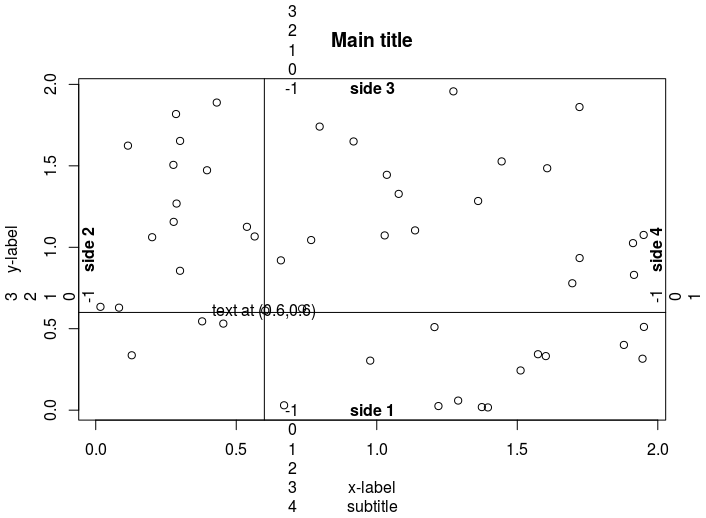
\includegraphics[width=\linewidth]{fig-5.png}
  \caption{La disposición de una gráfica estándar.}
  \label{fig:fig-5}
\end{figure}

Sin embargo, el hecho de que no se trace ningún gráfico no significa que no haya
pasado nada. El comando configura la región de trazado y los sistemas de
coordenadas como si realmente lo hubiera hecho. Para agregar los elementos de la
gráfica, evalúe lo siguiente:

\begin{lstlisting}[language=R]
> points(x,y)
> axis(1)
> axis(2,at=seq(0.2,1.8,0.2))
> box()
> title(main="Main title", sub="subtitle",xlab="x-label", ylab="y-label")
\end{lstlisting}

Observe cómo la llamada a \textt{axis} especifica un conjunto alternativo de
marcas de verificación (y etiquetas). Esta es una técnica común utilizada para
crear ejes especiales en un gráfico y también se puede utilizar para crear ejes
no equidistantes, así como ejes con etiquetado no numérico.

Trazar con \texttt{type="n"} es a veces una técnica útil porque tiene el efecto
secundario de dimensionar el área de la gráfica. Por ejemplo, para crear un
gráfico con diferentes colores para diferentes grupos, primero puede trazar
todos los datos con \texttt{type="n"}, asegurándose de que la región del gráfico
es lo suficientemente grande, y luego sumar los puntos para cada grupo usando
\texttt{points}. (Pasar un argumento vectorial para \texttt{col} es más
conveniente en este caso en particular.

%%%%%%%%%%%%%%%%%%%%%%%%%%%%%%%%%%%%%%%%%%%%%%%%%%%%%%%%%%%%%%%%%%%%%%%%%%%%%%%
\subsection{Utilizando \texttt{par}}
%%%%%%%%%%%%%%%%%%%%%%%%%%%%%%%%%%%%%%%%%%%%%%%%%%%%%%%%%%%%%%%%%%%%%%%%%%%%%%%

La función \texttt{par} permite un control increíblemente fino sobre los
detalles de un gráfico, aunque puede ser bastante confusa para los principiantes
(e incluso para los usuarios expertos a veces). La mejor estrategia puede ser
simplemente tratar de aprender algunos trucos útiles a la vez y de vez en cuando
tratar de resolver un problema en particular examinando la página de ayuda.

Algunos de los parámetros, pero no todos, también se pueden establecer mediante
parámetros a las funciones de dibujo, que también tienen algunos parámetros que
no se pueden establecer mediante \texttt{par}.  Cuando un parámetro se puede
establecer por ambos métodos, la diferencia es, generalmente que si algo se se
configuró mediante \texttt{par}, entonces permanecerá configurado
posteriormente.

La configuración de \texttt{par} permite controlar el ancho y el tipo de línea,
así como el tamaño de los caracteres y fuente de la letra, color, estilo de
cálculo de los ejes, tamaño de la gráfica y figuras, recortes, etc. Es posible
dividir una figura en varias subfiguras utilizando los parámetros \texttt{mfrow}
y \texttt{mfcol}.

Por ejemplo, los tamaños de margen predeterminados son algo más de 5, 4, 4 y 2
líneas.  Puede definir \texttt{par(mar=c(4,4,2,2)+0.1)} antes de graficar. Esto
quita una línea fuera del margen inferior y dos líneas fuera del margen superior
del gráfico, lo que reducirá la cantidad de espacios en blanco no utilizados
cuando no haya un título o subtítulo principal. Si se mira cuidadosamente, se
notará que la Figura \ref{fig:fig-5} tiene una región de trazado algo más
pequeña que las otras gráficas de este libro. Esto se debe a que las otras
gráficas se han realizado con márgenes reducidos por razones de composición
tipográfica.

Sin embargo, no tiene sentido describir los parámetros gráficos de forma
completa en este momento. Ya volveremos a ellos, cuando los utilicemos 
para gráficos específicos.

%%%%%%%%%%%%%%%%%%%%%%%%%%%%%%%%%%%%%%%%%%%%%%%%%%%%%%%%%%%%%%%%%%%%%%%%%%%%%%%
\subsection{Combinando gráficos}
%%%%%%%%%%%%%%%%%%%%%%%%%%%%%%%%%%%%%%%%%%%%%%%%%%%%%%%%%%%%%%%%%%%%%%%%%%%%%%%

Algunas consideraciones especiales surgen cuando usted desea poner varios
elementos juntos en la misma gráfica. Considere la posibilidad de superponer un
histograma de una densidad normal (consulte las Secciones 4.2 y 4.4.1 para
obtener información sobre los histogramas y la Sección 3.5.1 para la densidad).
Lo siguiente está cerca, pero no es lo suficientemente bueno (figura no
mostrada).

\begin{lstlisting}[language=R]
> x <- rnorm(100)
> hist(x,freq=F)
> curve(dnorm(x),add=T)
\end{lstlisting}

El parámetro \texttt{feq=F} en la llamada a \texttt{hist} nos asegura que el
histograma estará en términos de densidades en lugar de conteos absolutos.  La
función \texttt{curve} grafíca una expresión (en términos de x) y \texttt{add=T}
permite sobreponer la misma a una gráfica ya existente.  Por lo tanto, las cosas
parecieran estar configuradas correctamente, pero a veces la parte superior de
la función de densidad se corta. La razón es, por supuesto, que la altura de la
densidad normal no jugó ningún papel en el ajuste del eje \texttt{y} para el
histograma. No ayuda nada,  invertir el orden y dibujar la curva primero y
agregar el histograma luego, porque entonces las barras más altas podrían ser
las recortadas.

La solución es primero obtener la magnitud de los valores de \texttt{y} para ambos
elementos de la gráfica y hacer luego  que la gráfica sea lo suficientemente grande
como para contener ambos (Figura 2.2):

\begin{lstlisting}[language=R]
h <- hist(x, plot=F)
ylim <- range(0, h$density, dnorm(0))
hist(x, freq=F, ylim=ylim)
curve(dnorm(x), add=T)
\end{lstlisting}

\begin{figure}[H]
  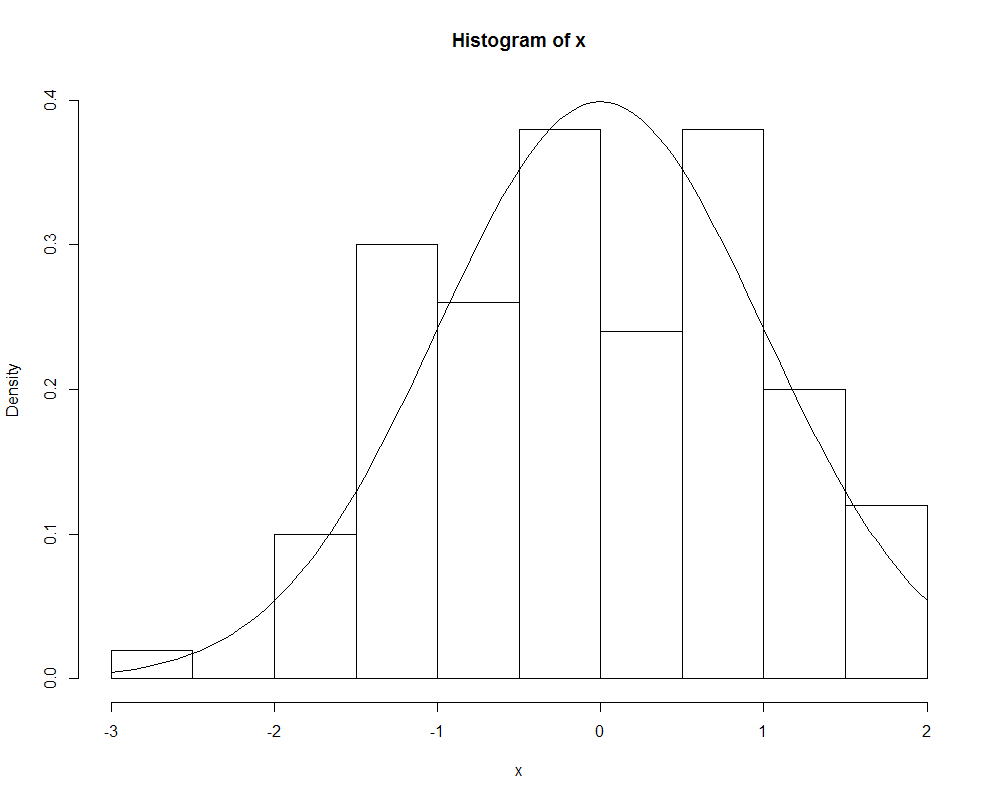
\includegraphics[width=\linewidth]{fig-6.png}
  \caption{Histograma con densidad normal superpuesta.}
  \label{fig:fig-6}
\end{figure}


\newpage

\section{R programming}
\subsection{Flow control} \label{flowcontrol}
\subsection{Classes and generic functions}

\section{Data entry}
\subsection{Leyendo desde un archivo de texto} \label{readtextfile}
\subsection{Further details on read.table}
\subsection{The data editor}
\subsection{Interfacing to other programs}
\section{Ejercicios}
